\section{Using Definite Integrals to Find Volume} \label{S:6.1.Volume}

\begin{goals}
\item How can we use a definite integral to find the volume of a three-dimensional solid of revolution that results from revolving a two-dimensional region about a particular axis?
\item In what circumstances do we integrate with respect to $y$ instead of integrating with respect to $x$?
\item What adjustments do we need to make if we revolve about a line other than the $x$- or $y$-axis?
\end{goals}

%-------------------------------
% SUBSECTION INTRODUCTION
%-------------------------------
\subsection*{Introduction}

\begin{marginfigure}[6cm] % MARGIN FIGURE
\includegraphics{figures/6_2_Intro.eps}
\caption{A right circular cylinder.} \label{F:6.1.Intro}
\end{marginfigure}

Just as we can use definite integrals to add up the areas of rectangular slices to find the exact area that lies between two curves, we can also employ integrals to determine the volume of certain regions that have cross-sections of a particular consistent shape.  As a very elementary example, consider a cylinder of radius $2$ and height $3$, as pictured in Figure~\ref{F:6.1.Intro}.  While we know that we can compute the area of any circular cylinder by the formula $V = \pi r^2 h$, if we think about slicing the cylinder into thin pieces, we see that each is a cylinder of radius $r = 2$ and height (thickness) $\triangle x$.  Hence, the volume of a representative slice is
$$V_{\small{\text{slice}}} = \pi \cdot 2^2 \cdot \triangle x.$$
Letting $\triangle x \to 0$ and using a definite integral to add the volumes of the slices, we find that 
$$V = \int_0^3 \pi \cdot 2^2 \, dx.$$
Moreover, since $\ds\int_0^3 4\pi \, dx = 12\pi$, we have found that the volume of the cylinder is $4\pi$.  The principal problem of interest in our upcoming work will be to find the volume of certain solids whose cross-sections are all thin cylinders (or washers) and to do so by using a definite integral.  To that end, we first consider another familiar shape in Preview Activity~\ref{PA:6.1}: a circular cone.

\input{previews/6.1.PA1} % PREVIEW

%--------------------------------------------
% SUBSECTION VOLUME OF A SOLID OF REVOLUTION
%--------------------------------------------
\subsection*{The Volume of a Solid of Revolution} \index{solid of revolution}

A solid of revolution is a three dimensional solid that can be generated by revolving one or more curves around a fixed axis.  For example, we can think of a circular cylinder as a solid of revolution:  in Figure~\ref{F:6.1.Intro}, this could be accomplished by revolving the area between the $x$-axis and the line segment from $(0,2)$ to $(3,2)$ about the $x$-axis.  Likewise, the circular cone in Figure~\ref{F:PA.6.1} is the solid of revolution generated by revolving the area between the $x$-axis and the portion of the line $y = 3 - \frac{3}{5}x$ from $x = 0$ to $x = 5$ about the $x$-axis.  It is particularly important to notice in any solid of revolution that if we slice the solid perpendicular to the axis of revolution, the resulting cross-section is circular.

We consider two examples to highlight some of the natural issues that arise in determining the volume of a solid of revolution.

\begin{example} \label{eg:6.1.1} % EXAMPLE
Find the volume of the solid of revolution generated when the region $R$ bounded by $y = 4-x^2$ and the $x$-axis is revolved about the $x$-axis.

\solution
First, we observe that $y = 4-x^2$ intersects the $x$-axis at the points $(-2,0)$ and $(2,0)$.  When we take the region $R$  that lies between the curve and the $x$-axis on this interval and revolve it about the $x$-axis, we get the three-dimensional solid pictured in Figure~\ref{F:6.1.Ex1}.

Taking a representative slice of the solid located at a value $x$ that lies between $x = -2$ and $x = 2$, we see that the thickness of such a slice is $\triangle x$ (which is also the height of the cylinder-shaped slice), and that the radius of the slice is determined by the curve $y = 4-x^2$.  Hence, we find that 
$$V_{\text{\small{slice}}} = \pi (4-x^2)^2 \triangle x,$$
since the volume of a cylinder of radius $r$ and height $h$ is $V = \pi r^2 h$.

Using a definite integral to sum the volumes of the representative slices, it follows that 
$$V = \int_{-2}^{2} \pi (4-x^2)^2 \, dx.$$
It is straightforward to evaluate the integral and find that the volume is $V = \frac{512}{15}\pi$.	
\end{example}

\begin{marginfigure}[-8cm] %MARGIN FIGURE
\includegraphics{figures/6_2_Ex1.eps}
\caption{The solid of revolution in Example~\ref{eg:6.1.1}.} \label{F:6.1.Ex1}
\end{marginfigure}

 %EXAMPLE

For a solid such as the one in Example~\ref{eg:6.1.1}, where each cross-section is a cylindrical disk, we first find the volume of a typical cross-section (noting particularly how this volume depends on $x$), and then we integrate over the range of $x$-values through which we slice the solid in order to find the exact total volume.  Often, we will be content with simply finding the integral that represents the sought volume; if we desire a numeric value for the integral, we typically use a calculator or computer algebra system to find that value.

The general principle we are using to find the volume of a solid of revolution generated by a single curve is often called the \emph{disk method}\index{disk method}.

\concept{Disk Method}{  % CONCEPT
If $y = r(x)$ is a nonnegative continuous function on $[a,b]$, then the volume of the solid of revolution generated by revolving the region bounded by the function and the $x$-axis about the $x$-axis over this interval is given by
$$V = \int_a^b \pi \left[ r(x) \right]^2 \, dx.$$
} %end CONCEPT

\begin{example} \label{eg:6.1.2} % EXAMPLE
Find the volume of the solid formed by revolving the region $R$ bounded by the curves $y=1/x$, $y=1/2$, and $y=1$ about the $y$-axis.

\solution Since the axis of rotation is vertical, we need to convert the function into a function of $y$ and use horizontal representative slices. Since $y=1/x$ defines the curve, we rewrite it as $x=1/y$. %The bound $x=1$ corresponds to the $y$-bound $y=1$, and the bound $x=2$ corresponds to the $y$-bound $y=1/2$. 

Thus we are rotating the curve $x=1/y$, from $y=1/2$ to $y=1$ about the $y$-axis to form a solid. The curve and sample differential element are sketched in Figure~\ref{F:6-1-EG2}-(a), with a full sketch of the solid in Figure~\ref{F:6-1-EG2}-(b).

We integrate to find the volume:
\begin{align*}
V &= \pi\int_{1/2}^1 \frac{1}{y^2}\ dy \\
	&= -\frac{\pi}y\Big|_{1/2}^1 \\
	&= \pi\ \text{units}^3.
\end{align*}		
\end{example}

\begin{marginfigure}[0cm] %MARGIN FIGURE
\subfloat[]{\margingraphics{figures/figdisk1a}}

\subfloat[]{\margingraphics{figures/figdisk2a}}
\caption{Sketching the solid in Example \ref{eg:6.1.2}.}
\label{F:6-1-EG2}
\end{marginfigure} %EXAMPLE

A different type of solid can emerge when two curves are involved, as we see in the following example.

\begin{marginfigure}[2cm] %MARGIN FIGURE
\margingraphics{figures/6_2_Ex2.eps}
\caption{At left, the solid of revolution in Example~\ref{eg:6.1.3}.  At right, a typical slice with inner radius $r(x)$ and outer radius $R(x)$.} \label{F:6.1.Eg3}
\end{marginfigure}

\begin{example} \label{eg:6.1.3} % EXAMPLE
Find the volume of the solid of revolution generated when the finite region $R$ that lies between $y = 4-x^2$ and $y = x+2$ is revolved about the $x$-axis.


\solution
First, we must determine where the curves $y = 4-x^2$ and $y = x+2$ intersect.  Substituting the expression for $y$ from the second equation into the first equation, we find that $x + 2 = 4-x^2$.  Rearranging, it follows that
$$x^2 + x - 2 = 0,$$
and the solutions to this equation are $x = -2$ and $x = 1$.  The curves therefore cross at $(-2,0)$ and $(1,3)$.

When we take the region $R$  that lies between the curves and revolve it about the $x$-axis, we get the three-dimensional solid pictured at left in Figure~\ref{F:6.1.Eg3}.

Immediately we see a major difference between the solid in this example and the one in Example~\ref{eg:6.1.2}:  here, the three-dimensional solid of revolution isn't ``solid'' in the sense that it has open space in its center.  If we slice the solid perpendicular to the axis of revolution, we observe that in this setting the resulting representative slice is not a solid disk, but rather a \emph{washer}, as pictured at right in Figure~\ref{F:6.1.Eg3}.  Moreover, at a given location $x$ between $x = -2$ and $x = 1$, the small radius $r(x)$ of the inner circle is determined by the curve $y = x+2$, so $r(x) = x+2$.  Similarly, the big radius $R(x)$ comes from the function $y = 4-x^2$, and thus $R(x) = 4-x^2$.

Thus, to find the volume of a representative slice, we compute the volume of the outer disk and subtract the volume of the inner disk.  Since
$$\pi R(x)^2 \triangle x - \pi r(x)^2 \triangle x = \pi [ R(x)^2 - r(x)^2] \triangle x,$$
it follows that the volume of a typical slice is
$$V_{\text{\small{slice}}} = \pi [ (4-x^2)^2 - (x+2)^2 ] \triangle x.$$
Hence, using a definite integral to sum the volumes of the respective slices across the integral, we find that
$$V = \int_{-2}^1 \pi[ (4-x^2)^2 - (x+2)^2 ] \, dx.$$
Evaluating the integral, the volume of the solid of revolution is $\ds V = \frac{108}{5}\pi$.
\end{example} % EXAMPLE

The general principle we are using to find the volume of a solid of revolution generated by revolving a region bounded by two curves is often called the \emph{washer method}\index{washer method}.

\concept{Washer Method}{ % CONCEPT
If $y = R(x)$ and $y = r(x)$ are nonnegative continuous functions on $[a,b]$ that satisfy $R(x) \ge r(x)$ for all $x$ in $[a,b]$, then the volume of the solid of revolution generated by revolving the region between them about the $x$-axis over this interval is given by
$$V = \int_a^b \pi [R(x)^2 - r(x)^2] \, dx.$$
} %end CONCEPT

\input{activities/6.1.Act1} % ACTIVITY

%--------------------------------------------
% SUBSECTION REVOLVING ABOUT THE Y-AXIS
%--------------------------------------------
\subsection*{Revolving about the $y$-axis}

As seen in Activity~\ref{A:6.1.1}, problem~(e), the problem changes considerably when we revolve a given region about the $y$-axis.  Foremost, this is due to the fact that representative slices now have thickness $\triangle y$, which means that it becomes necessary to integrate with respect to $y$.  Let's consider a particular example to demonstrate some of the key issues.

\begin{example} \label{eg:6.1.4} % EXAMPLE
Find the volume of the solid of revolution generated when the finite region $R$ that lies between $y = \sqrt{x}$ and $y = x^4$ is revolved about the $y$-axis.

\solution
We observe that these two curves intersect when $x = 1$, hence at the point $(1,1)$.  When we take the region $R$ that lies between the curves and revolve it about the $y$-axis, we get the three-dimensional solid pictured at left in Figure~\ref{F:6.2.Ex3}.

Now, it is particularly important to note that the thickness of a representative slice is $\triangle y$, and that the slices are only cylindrical washers in nature when taken perpendicular to the $y$-axis.  Hence, we envision slicing the solid horizontally, starting at $y = 0$ and proceeding up to $y = 1$.  Because the inner radius is governed by the curve $y = \sqrt{x}$, but from the perspective that $x$ is a function of $y$, we solve for $x$ and get $x = y^2 = r(y)$.  In the same way, we need to view the curve $y = x^4$ (which governs the outer radius) in the form where $x$ is a function of $y$, and hence $x = \sqrt[4]{y}$.  Therefore, we see that the volume of a typical slice is 
$$V_{\mbox{\small{slice}}} = \pi [R(y)^2 - r(y)^2] = \pi[\sqrt[4]{y}^2 - (y^2)^2] \triangle y.$$
Using a definite integral to sum the volume of all the representative slices from $y = 0$ to $y = 1$, the total volume is
$$V = \int_{y=0}^{y=1} \pi \left[ \sqrt[4]{y}^2 - (y^2)^2 \right] \, dy.$$
It is straightforward to evaluate the integral and find that $\ds V = \frac{7}{15} \pi$.
\end{example}

\begin{marginfigure}[-12cm] %MARGIN FIGURE
\margingraphics{figures/6_2_Ex3.eps}
\caption{At left, the solid of revolution in Example~\ref{eg:6.1.4}.  At right, a typical slice with inner radius $r(y)$ and outer radius $R(y)$.} \label{F:6.2.Ex3}
\end{marginfigure}

 % EXAMPLE

\input{activities/6.1.Act2} % ACTIVITY

%--------------------------------------------
% SUBSECTION REVOLVING ABOUT OTHER LINES
%--------------------------------------------
\subsection*{Revolving about horizontal and vertical lines other than the coordinate axes}

Just as we can revolve about one of the coordinate axes ($y = 0$ or $x = 0$), it is also possible to revolve around any horizontal or vertical line.  Doing so essentially adjusts the radii of cylinders or washers involved by a constant value.  A careful, well-labeled plot of the solid of revolution will usually reveal how the different axis of revolution affects the definite integral we set up.  Again, an example is instructive.

\begin{example} \label{eg:6.1.5} % EXAMPLE
Find the volume of the solid of revolution generated when the finite region $S$ that lies between $y = x^2$ and $y = x$ is revolved about the line $y = -1$.

\solution 
Graphing the region between the two curves in the first quadrant between their points of intersection ($(0,0)$ and $(1,1)$) and then revolving the region about the line $y = -1$, we see the solid shown in Figure~\ref{F:6.2.Ex4}.  Each slice of the solid perpendicular to the axis of revolution is a washer, and the radii of each washer are governed by the curves $y = x^2$ and $y = x$.  But we also see that there is one added change:  the axis of revolution adds a fixed length to each radius.  In particular, the inner radius of a typical slice, $r(x)$, is given by $r(x) = x^2 + 1$, while the outer radius is $R(x) = x+1$.  Therefore, the volume of a typical slice is
$$V_{\mbox{\small{slice}}} = \pi[ R(x)^2 - r(x)^2 ] \triangle x = \pi \left[ (x+1)^2 - (x^2 + 1)^2 \right] \triangle x.$$
Finally, we integrate to find the total volume, and 
$$V = \int_0^1  \pi \left[ (x+1)^2 - (x^2 + 1)^2 \right] \, dx = \frac{7}{15} \pi.$$
\end{example}

\begin{marginfigure}[-10cm] %MARGIN FIGURE
\margingraphics{figures/6_2_Ex4.eps}
\caption{The solid of revolution described in Example~\ref{eg:6.1.5}.} \label{F:6.2.Ex4}
\end{marginfigure}

 % EXAMPLE

\input{activities/6.1.Act3} % ACTIVITY

%--------------------------------------------
% SUBSECTION VOLUMES OF OTHER SOLIDS
%--------------------------------------------
\subsection*{Volumes of Other Solids}

Given an arbitrary solid, we can \textit{approximate} its volume by cutting it into $n$  thin slices. When the slices are thin, each slice can be approximated by a right cylinder with known cross-sectional area . Thus the volume of each slice is approximately its cross-sectional area $\times$ thickness. (These slices are the differential elements.)

By orienting a solid along the $x$-axis, we can let $A(x_i)$ represent the cross-sectional area
of the $i\,^\text{th}$ slice, and let $\dx_i$ represent the thickness of this slice (the thickness is a small change in $x$). The total volume of the solid is approximately:
\begin{align*} \text{Volume} &\approx \sum_{i=1}^n \Big[\text{Area}\ \times\ \text{thickness}\Big] \\
&= \sum_{i=1}^n A(x_i)\dx_i.
\end{align*}
	
Recognize that this is a Riemann Sum. By taking a limit (as the thickness of the slices goes to $0$) we can find the volume exactly. 

\concept{Volume By Cross-Sectional Area} % CONCEPT
{The volume $V$ of a solid, oriented along the $x$-axis with cross-sectional area $A(x)$ from $x=a$ to $x=b$, is \index{integration!volume!cross-sectional area}
$$V = \int_a^b A(x)\ dx.$$
} %end CONCEPT

\begin{marginfigure}[6cm] %MARGIN FIGURE
\margingraphics{figures/figcross_area1}
\caption{Orienting a pyramid along the $x$-axis in Example~\ref{eg:6.1.6}.} \label{F:6.1.Ex6}
\end{marginfigure}

\begin{example} \label{eg:6.1.6} % EXAMPLE
Find the volume of a pyramid with a square base of side length $10$ in and a height of $5$ in.

\solution There are many ways to ``orient'' the pyramid along the $x$-axis; Figure~\ref{F:6.1.Ex6} gives one such way, with the pointed top of the pyramid at the origin and the $x$-axis going through the center of the base.

Each cross section of the pyramid is a square; this is a sample differential element. To determine its area $A(x)$, we need to determine the side lengths of the square.

When $x=5$, the square has side length $10$; when $x=0$, the square has side length $0$. Since the edges of the pyramid are lines, it is easy to figure that each cross-sectional square has side length $2x$, giving $A(x) = (2x)^2=4x^2$. We have 
\begin{align*} 
V &= \int_0^5 4x^2\ dx\\
&= \frac43x^3\Big|_0^5 \\
&=\frac{500}{3}\ \text{in}^3 \approx 166.67\ \text{in}^3.
\end{align*}
We can check our work by consulting the general equation for the volume of a pyramid: %(see the back cover under ``Volume of A General Cone''): 

$$\frac13 \times \text{area of base}\times \text{height.}$$

Certainly, using this formula from geometry is faster than our new method, but the calculus-based method can be applied to much more than just cones.
\end{example}



 % EXAMPLE

%-------------
% SUMMARY
%-------------
\begin{summary}
  \item We can use a definite integral to find the volume of a three-dimensional solid of revolution that results from revolving a two-dimensional region about a particular axis by taking slices perpendicular to the axis of revolution which will then be circular disks or washers.
  \item If we revolve about a vertical line and slice perpendicular to that line, then our slices are horizontal and of thickness $\triangle y$. This leads us to integrate with respect to $y$, as opposed to with respect to $x$ when we slice a solid vertically.
  \item If we revolve about a line other than the $x$- or $y$-axis, we need to carefully account for the shift that occurs in the radius of a typical slice.  Normally, this shift involves taking a sum or difference of the function along with the constant connected to the equation for the horizontal or vertical line; a well-labeled diagram is usually the best way to decide the new expression for the radius.
\end{summary}

\clearpage

%--------------
% EXERCISES
%--------------
\begin{adjustwidth*}{}{-2.25in}
\textbf{{\large Exercises}}
\setlength{\columnsep}{25pt}
\begin{multicols*}{2}
\noindent Terms and Concepts \small
\begin{enumerate}[1)]
\item T/F: A solid of revolution is formed by revolving a shape around an axis.
\item In your own words, explain how the Disk and Washer Methods are related.
\item Explain the how the units of volume are found in the integral: if $A(x)$ has units of in$^2$, how does $\int A(x)\ dx$ have units of in$^3$?
\end{enumerate} 

\noindent {\normalsize Problems} \small

\noindent{\bf In Exercises 4--7, a region of the Cartesian plane is shaded. Use the Disk/Washer Method to find the volume of the solid of revolution formed by revolving the region about the $x$-axis.}

\begin{enumerate}[1),resume]
\item \begin{minipage}{\linewidth}\centering\includegraphics{figures/fig07_02_ex_04}\end{minipage}

\item \begin{minipage}{\linewidth}\centering\includegraphics{figures/fig07_02_ex_05}\end{minipage}

\item \begin{minipage}{\linewidth}\centering\includegraphics{figures/fig07_02_ex_06}\end{minipage}

\item \begin{minipage}{\linewidth}\centering\includegraphics{figures/fig07_02_ex_07}\end{minipage}
\end{enumerate}

\noindent{\bf In Exercises 8-11, a region of the Cartesian plane is shaded. Use the Disk/Washer Method to find the volume of the solid of revolution formed by revolving the region about the $y$-axis.}

\begin{enumerate}[1),resume]
\item \begin{minipage}{\linewidth}\centering\includegraphics{figures/fig07_02_ex_08}\end{minipage}

\item \begin{minipage}{\linewidth}\centering\includegraphics{figures/fig07_02_ex_09}\end{minipage}

\item \begin{minipage}{\linewidth}\centering\includegraphics{figures/fig07_02_ex_10}\end{minipage}
\end{enumerate}

%------------------------------------------
% END OF EXERCISES ON FIRST PAGE
%------------------------------------------
\end{multicols*}
\end{adjustwidth*}

\clearpage

\begin{adjustwidth*}{}{-2.25in}
\setlength{\columnsep}{25pt}
\begin{multicols*}{2}\small

\begin{enumerate}[1),start=11]
\item \begin{minipage}{\linewidth}\centering\includegraphics{figures/fig07_02_ex_11}\end{minipage}

(Hint: Integration By Parts will be necessary, twice. First let $u = \arccos^2x$, then let $u=\arccos x$.)
\end{enumerate}

\vspace{.25cm}

\noindent{\bf In Exercises 12--17, a region of the Cartesian plane is described. Use the Disk/Washer Method to find the volume of
the solid of revolution formed by rotating the region about each of the given axes.}

\begin{enumerate}[1),resume]
\item Region bounded by: $y=\sqrt{x}$, $y=0$ and $x=1$.

Rotate about:

\noindent%
\begin{minipage}[t]{.5\linewidth}
\begin{enumerate}
\item		the $x$-axis
\item		$y=1$
\end{enumerate}
\end{minipage}
\begin{minipage}[t]{.5\linewidth}
\begin{enumerate}\addtocounter{enumii}{2}
\item		the $y$-axis
\item		$x=1$
\end{enumerate}
\end{minipage}

\item Region bounded by: $y=4-x^2$ and $y=0$.

Rotate about:

\noindent%
\begin{minipage}[t]{.5\linewidth}
\begin{enumerate}
\item		the $x$-axis
\item		$y=4$
\end{enumerate}
\end{minipage}
\begin{minipage}[t]{.5\linewidth}
\begin{enumerate}\addtocounter{enumii}{2}
\item		$y=-1$
\item		$x=2$
\end{enumerate}
\end{minipage}

\item The triangle with vertices $(1,1)$, $(1,2)$ and $(2,1)$.

Rotate about:

\noindent%
\begin{minipage}[t]{.5\linewidth}
\begin{enumerate}
\item		the $x$-axis
\item		$y=2$
\end{enumerate}
\end{minipage}
\begin{minipage}[t]{.5\linewidth}
\begin{enumerate}\addtocounter{enumii}{2}
\item		the $y$-axis
\item		$x=1$
\end{enumerate}
\end{minipage}

\item Region bounded by $y=x^2-2x+2$ and $y=2x-1$.

Rotate about:

\noindent%
\begin{minipage}[t]{.5\linewidth}
\begin{enumerate}
\item		the $x$-axis
\item		$y=1$
\end{enumerate}
\end{minipage}
\begin{minipage}[t]{.5\linewidth}
\begin{enumerate}\addtocounter{enumii}{2}
%\item		the $y$-axis
\item		$y=5$
\end{enumerate}
\end{minipage}

\item Region bounded by $y=1/\sqrt{x^2+1}$, $x=-1$, $x=1$ and the $x$-axis.

Rotate about:

\noindent%
\begin{minipage}[t]{.5\linewidth}
\begin{enumerate}
\item		the $x$-axis
\item		$y=1$
\end{enumerate}
\end{minipage}
\begin{minipage}[t]{.5\linewidth}
\begin{enumerate}\addtocounter{enumii}{2}
%\item		the $y$-axis
\item		$y=-1$
\end{enumerate}
\end{minipage}

\item Region bounded by $y=2x$, $y=x$ and $x=2$.

Rotate about:

\noindent%
\begin{minipage}[t]{.5\linewidth}
\begin{enumerate}
\item		the $x$-axis
\item		$y=4$
\end{enumerate}
\end{minipage}
\begin{minipage}[t]{.5\linewidth}
\begin{enumerate}\addtocounter{enumii}{2}
\item		the $y$-axis
\item		$x=2$
\end{enumerate}
\end{minipage}

\end{enumerate}

\noindent{\bf In Exercises 18--21, a solid is described. Orient the solid along the $x$-axis such that a cross-sectional area function $A(x)$ can be obtained, then find the volume of the solid.}

\begin{enumerate}[1),resume]
\item A right circular cone with height of 10 and base radius of 5. \label{ex_07_02_ex_18}

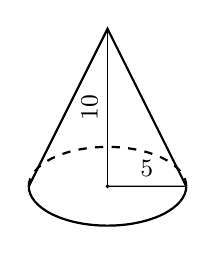
\begin{tikzpicture}[scale=.5]
\begin{scope}[xscale=2]
%\draw [thick](0,0) circle (1);
\draw [thick] (-1,0) arc (180:360:1);
\draw [thick,dashed] (1,0) arc (0:180:1);
\end{scope}

\draw [fill=black] (0,0) circle (1pt) -- node [pos=.5,above] {\small 5} (2,0);
\draw (0,0) -- node [pos=.5,rotate=90,above] {\small 10} (0,4);
\draw [thick] (-2,0) -- (0,4)-- (2,0);
\end{tikzpicture}

\item A skew right circular cone with height of 10 and base radius of 5. (Hint: all cross-sections are circles.)

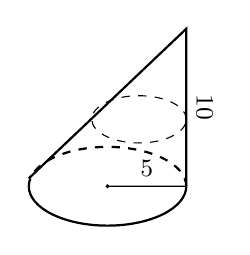
\begin{tikzpicture}[scale=.5]
\begin{scope}[xscale=2]
%\draw [thick](0,0) circle (1);
\draw [thick] (-1,0) arc (180:360:1);
\draw [thick,dashed] (1,0) arc (0:180:1);
\draw [dashed] (.4,1.7) circle (.6);
\end{scope}

\draw [fill=black] (0,0) circle (1pt) -- node [pos=.5,above] {\small 5} (2,0);
%\draw (0,0) -- node [pos=.5,rotate=90,above] {\small 10} (0,4);
\draw [thick] (-2,0.2) -- (2,4)-- node [pos=.5,rotate=-90,above] {\small 10}(2,0);
\end{tikzpicture}

\item A right triangular cone with height of 10 and whose base is a right, isosceles triangle with side length 4.

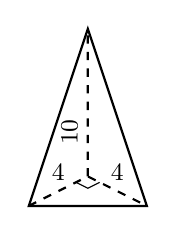
\begin{tikzpicture}[scale=.75]
\draw [thick](-1,0) -- (1,0) -- (0,3)--cycle;
\draw [thick,dashed] (-1,0) --  node [pos=.5,above] {\small 4} (0,.5) -- node [pos=.5,above] {\small 4} (1,0)
											(0,.5)-- node [pos=.3,above,rotate=90] {\small 10} (0,3);
\draw (-.2,.4) -- (0,.3) -- (.2,.4);
\end{tikzpicture}

\item A solid with length 10 with a rectangular base and triangular top, wherein one end is a square with side length 5 and the other end is a triangle with base and height of 5.

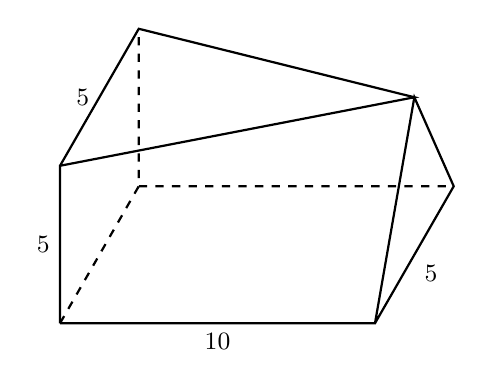
\begin{tikzpicture}[x={(1,0)},z={(0,1)},y={(.5,.87)},scale=.4]

\draw [thick] (0,0,0) -- node[pos=.5,below] {\small 10} (10,0,0) -- (10,2.5,5) -- (10,5,0) -- node [pos=.5,below right] {\small 5} (10,0,0)
							(0,0,0) -- node [pos=.5,left] {\small 5} (0,0,5) -- (10,2.5,5) -- (0,5,5) -- node [pos=.5,left] {\small 5} (0,0,5);
							
\draw [thick,dashed] (0,0,0) -- (0,5,0) -- (0,5,5)
										(0,5,0) -- (10,5,0);



\end{tikzpicture}

\end{enumerate}

%---------------------------------------------
% END OF EXERCISES ON SECOND PAGE
%---------------------------------------------
\end{multicols*}
\end{adjustwidth*}

\afterexercises 

\cleardoublepage